\documentclass[10pt,a4paper]{article}
%\usepackage[english,spanish]{babel}

\usepackage{indentfirst}
\usepackage{anysize} % Soporte para el comando \marginsize
%\marginsize{1.5cm}{1.5cm}{0.5cm}{1cm}
\marginsize{2,5cm}{1,8cm}{4cm}{1,7cm}
\usepackage[psamsfonts]{amssymb}
\usepackage{amssymb}
\usepackage{amsfonts}
\usepackage{amsmath}
\usepackage{multirow} % para las tablas
\usepackage{amsthm}
\usepackage{stackrel}
\usepackage{graphicx}
\usepackage[colorinlistoftodos]{todonotes}
%Color a las referencias
\usepackage[colorlinks=true, allcolors=blue]{hyperref}
\usepackage[spanish]{babel}
\selectlanguage{spanish}
\usepackage[utf8]{inputenc} 
\usepackage{multicol}
\renewcommand{\thepage}{}
\columnsep=7mm

%%%%%%%%%%%%%%%%%%%%%%%%%%%%%%%%%%%%%%%%
\newtheorem{definicion}{Definici\'on}[section]
\newtheorem{teorema}{Teorema}[section]
\newtheorem{prueba}{Prueba}[section]
\newtheorem{prueba*}{Prueba}[section]
\newtheorem{corolario}{Corolario}[section]
\newtheorem{observacion}{Observaci\'on}[section]
\newtheorem{lema}{Lema}[section]
\newtheorem{ejemplo}{Ejemplo}[section]
\newtheorem{solucion*}{Soluci\'on}[section]
\newtheorem{algoritmo}{Algoritmo}[section]
\newtheorem{proposicion}{Proposici\'on}[section]

\linespread{1.4} \sloppy

\newcommand{\R}{\mathbf{R}}
\newcommand{\N}{\mathbf{N}}
\newcommand{\C}{\mathbb{C}}
\newcommand{\Lr}{\mathcal{L}}
\newcommand{\fc}{\displaystyle\frac}
\newcommand{\ds}{\displaystyle}

\DeclareMathOperator{\Dom}{Dom}

%%%%%%%%%%%%%%%%%%%%%%%%%%%%%%%%%%%%%%%%

\renewcommand{\thefootnote}{\fnsymbol{footnote}}
\usepackage{url}
\usepackage{hyperref}

\begin{document}
	\begin{center}
		{\Large \textbf{PREDICCIÓN DE LA CONCENTRACIÓN EN UNA REACCIÓN QUÍMICA}}
	\end{center}
	\begin{center}
		Lázaro-Camasca$^{1}$, Ponce-Pinedo$^{2}$, Sarria-Palacios$^{3}$, Loayza-Pizarro$^{4}$\vskip5pt
		{\it Facultad de Ciencias$^1$, Universidad Nacional de Ingenier\'{\i}a$^1$\\}\vskip5pt
		Email: elazaroc@uni.pe$^{1}$, victor.ponce.p@uni.pe$^{2}$,esarriap@uni.pe$^{3}$, fernando.loayza.p@uni.pe$^{4}$
	\end{center}
	%\maketitle 
	\vspace*{0.4cm}
	
	\begin{abstract}
		
		En diversos campos de la ingenieria y ciencia se necesita obtener datos a partir de casos experimentales. Las reacciones quimicas no son ajenas a esta, por ello conocer las concentraciones de estas ayuda a muchos profesionales. Los químicos y biólogos miden las cantidades agentes contaminantes para determinar los niveles de \textbf{contaminación en el ambiente}. En la industria farmacéutica los laboritaristas miden las cantidades de sustancias necesarias para preparar medicamentos; todas estas de concentración determinada y de cuya exacta preparación \textbf{depende de la vida y la pronta recuperación de cientos de miles de enfermos}. En las industrias alimentarias los ingenieros miden las cantidades de sustancias, con el propósito de \textbf{incrementar sus ingresos economicos}. Este documento proporciona una comparación entre los metodos de ajuste exacto(Interpolación) y minimos cuadrados(Aproximación Funcional), además sugiere que metodo o la combinación de ambos predice con mayor exactitud la concentracion del producto.
		
	\end{abstract}
	
	
	\begin{quotation}
		{\small
			\noindent\textbf{Palabras Clave:} \\ 
			Casos experimentales, Concentración, Contaminacion Ambiental, Industrias, Interpolación, Aproximación Funcional.
		}
	\end{quotation}
	
	
	\renewcommand{\abstractname}{Abstract}
	
	\begin{abstract}
		\noindent Falta
	\end{abstract}
	
	
	\begin{quotation}
		{\small
			\textbf{Keywords:} \\ 
		}
	\end{quotation}
	
	
	\pagebreak
	
	\begin{multicols}{2}
		
		\begin{center}
			{\large \bf 1. INTRODUCCIÓN}
		\end{center}
		
		En las reacciones quimicas la velocidad de la reacción dependen de diversos parametros tales como la temperatura, la presión, la concentracion de los reactivos estos al ser variados aumentan o disminuyen la velocidad.
		
		\noindent Las industrias se interesan grandemente en que las reacciones químicas se lleven a cabo rápidadmente, para \textbf{ahorrar tiempo y dinero}. Es por esto que  encontrar las concentraciones en un tiempo especifico es muy complicado, una posible solución seria contar con un dispositivo que registre en tiempo real las concentraciones, pero esto seria muy costoso. Una alternativa para esto es
		el uso de la matematica en concreto el uso de metodos numericos.
		
		\noindent Por ello en presente trabajo se describe la obtención de una función que caracteriza la concentración de producto de una reacción química en función del tiempo. Esta función será calculada mediante métodos de interpolación polinomial y minimos cuadrados a partir puntos tabulados que han sido obtenidos de manera experimental.\\
		
		
		\begin{center}
			{\large \bf 2. CONCEPTOS PREVIOS}
		\end{center}
		
		\noindent {\large \bf 2.1. Reacciones Química}
		
		\noindent Es un proceso en el que dos o más sustancias (reactantes) se transforman en una o más sustancias (productos). Estas reacciones deben satisfacer la ley de la conservación de la materia.
		
		\begin{center}
			$aA  +  bB  ->  cC  +  dD$
		\end{center}
		
		
		\noindent {\large \bf 2.1. Velocidad Instantánea de Reacción}
		
		\noindent Expresa el cambio de la concentración de un reactivo o de un producto por unidad de tiempo (concentración/tiempo).\\
		
		\begin{center}
			{\scriptsize
				$v = \dfrac{-d[A]}{a*d[t]} = \dfrac{-d[B]}{b*d[t]} = \dfrac{-d[C]}{c*d[t]} = \dfrac{-d[D]}{d*d[t]}$ \\ 
				
			}
		\end{center}
		
		\vspace*{0.4cm}
		
		\noindent {\large \bf 2.2. Interpolación polinomial}
		
		\noindent Planteamos tres problemas relacionados con la aproximación de funciones
		
		Primero, suponga que tenemos una tabla de valores numéricos de una función:
		
		\begin{center}
			\begin{tabular}{ c|c|c|c|c }
				
				$x$ & $x_0$ & $x_1$ & $...$ & $x_n$ \\ \hline
				$y$ & $y_0$ & $y_1$ & $...$ & $y_n$
			\end{tabular}
		\end{center}
		
		¿Es posible encontrar una fórmula simple y conveniente que reproduzca los puntos dados exactamente?
		
		El segundo problema es similar, pero se supone que la tabla de valores numéricos dada está contaminada por errores, como puede ocurrir si los valores provienen de un experimento de física. Ahora nos preguntamos por una fórmula que represente los datos (aproximadamente) y, si es posible, filtre los errores.
		
		Como un tercer problema, una función f está dada, quizás en la forma de un procedimiento computacional, pero es costoso evaluarla. En este caso, nos preguntamos por otra función g que sea simple de evaluar y produzca una aproximación razonable a f. A veces en este problema, queremos que g se aproxime a f con precisión total de máquina.
		
		En todos estos problemas, se puede obtener una función simple p que represente o aproxime a la tabla o función f dadas. La representación p siempre se puede tomar como un polinomio, aunque también se pueden usar muchos otros tipos de funciones simples. Una vez que se ha obtenido una función simple p, se puede usar en lugar de f en muchas situaciones. Por ejemplo, la integral de f se podría estimar con la integral de p y, generalmente, esta última debe ser más fácil de evaluar
		
		\noindent {\large \bf 2.2.1 Polinomios de Lagrange}
		\vspace*{0.2cm}
		
		\noindent Suponga que queremos interpolar funciones arbitrarias en un conjunto de nodos fijos $x_0, x_1, . . . , x_n$.
		Primero definimos un sistema de $n + 1$ polinomios especiales de grado n conocidos como \textbf{polinomios
			cardinales} en la teoría de interpolación. Éstos se denotan por $L_0, L_1, . . . , L_n$ y tienen la propiedad:
		\begin{center}
			
			$L_i(x_j) = \gamma_{ij}=\left \{ \begin{matrix} 0 & \mbox{si} i\not=j \\ 1 & \mbox{si } i=j\end{matrix}\right$
		\end{center}
		
		\noindent Una vez que están disponibles, podemos interpolar cualquier función $f$ por la \textbf{forma de Lagrange de interpolación polinomial}:
		\begin{center}
			$p_n(x) = \displaystyle\sum_{i=0}^n L_i(x) f(x_i)$
		\end{center}
		
		\noindent Esta función $p_n$, al ser una combinación lineal de los polinomios $L_i$, es en sí misma un polinomio de grado a lo más $n$. Además, cuando evaluamos $p_n$ en $x_i$ obtenemos $f(x_j)$:
		\begin{center}
			$p_n(x_j) = \displaystyle\sum_{i=0}^n L_i(x_j) f(x_i) = L_j(x_j)f(x_j) = f(x_j)$
		\end{center}
		
		\noindent Por tanto, $p_n$ es el polinomio de interpolación para la función $f$ en los nodos $x_0, x_1, . . . , x_n$. Ahora sólo resta escribir la fórmula para el polinomio cardinal $i$, que es
		
		\begin{center}
			$L_i(x) = \displaystyle\prod_{j\not=i,j=0}^n (\frac{x-x_j}{x_i-x_j})$
		\end{center}
		
		Esta fórmula indica que $L_i(x)$ es el producto de n factores lineales:
		
		\vspace*{0.2cm}
		
		
		$L_i(x) = (\frac{x-x_0}{x_i-x_0}) (\frac{x-x_1}{x_i-x_1})...(\frac{x-x_{i_1}}{x_i-x_{i-1}})(\frac{x-x_{i+1}}{x_i-x_{i+1}})...(\frac{x-x_n}{x_i-x_n}) $
		
		\vspace*{0.2cm}
		
		\noindent Los denominadores son sólo números; la variable $x$ se presenta únicamente en los numeradores. Por tanto, $i$ es un polinomio de grado $n$. Observe que cuando $L_i(x)$ se evalúa en $x = x_i$, cada factor en la ecuación anterior será $1$. Por tanto, $L_i(x_i) = 1$. Pero cuando se evalúa $L_i(x)$ en cualquier otro nodo, digamos, $x_j$, uno de los factores en la ecuación anterior será $0$ y $L_i(x_j) = 0$ para $i \not= j$.
		\vspace*{0.2cm}
		
		\noindent {\large \bf 2.2.2 Método de Newton}
		
		\vspace*{0.2cm}
		
		\noindent Supóngase que se tiene una función dada en forma tabular como se presenta a continuación
		
		\begin{center}
			\begin{tabular}{ c|c|c|c|c }
				\hline
				$Puntos$ & 0 & 1 & $...$ & n\\ \hline
				$x$ & $x_0$ & $x_1$ & $...$ & $x_n$  \\
				$f(x)$ & $f[x_0]$ & $f[x_1]$  &$...$ & $f[x_n]$ \\ \hline
				
			\end{tabular}
		\end{center}
		
		y que se desea aproximarla preliminarmente con un polinomio de primer grado que pasa, por ejemplo, por los puntos $(0)$ y $(1)$. Sea además dicho polinomio de la forma:
		\begin{center}
			$p(x) = a_0 + a_1(x-x_0)$ ...... (*)
		\end{center}
		donde $x_0$ es la abscisa del punto $(0)$ y $a_0$,$a_1$ son constantes por determinar. Para encontrar el valor de $a_0$ se hace $x=x_0$, de donde $a_0 = p(x_0) = f[x_0]$, y fin de encontrar el valor de $a_1$ se hae $x = x_1$, de donde $a_1 = (f[x_1]-f[x_0])/(x_1-x_0)$, o sea la primera diferencia dividida $f[x_1,x_0]$.
		
		Al sustituir los valores de estas constantes en la ecuación (*) ésta queda
		\begin{center}
			$p(x) = f[x_0] + (x - x_0)f[x_0,x_1]$
		\end{center}
		o sea un polinomio de primer grado en términos de diferencias divididas.
		Y si ahora se desea aproximar la función tabular con un polinomio de segundo grado que pase por los puntos (0), (1) y (2) y que tenga la forma:
		\begin{center}
			$p_2(x) = a_0 + a_1(x-x_0) + a_2(x-x0)(x-x_1)$
		\end{center}
		generalizando se puede formar para $p_n$.
		
		\noindent Una observación muy importante acerca de $p_n$ es que los coeficientes $a_0, a_1,. ..$, no dependen de $n$. En otras palabras, $p_n$ se obtiene de $p_{n-1}$ sumando un término más, sin alterar los coeficientes que ya están en $p_{n-1}$. Este es porque comenzamos esperando que pn pudiera expresarse en la forma:
		\begin{center}
			$p_n(x) = p_{n-1}(x) + a_n(x-x_0)...(x-x_{n-1})$
		\end{center}
		
		
		y descubrimos que esto de hecho era posible.
		
		\noindent Una forma de determinar sistemáticamente los coeficientes desconocidos $a_0, a_1, . . . , a_n$ es hacer $x$ igual a $x_0, x_1, . . . , x_n$ en la forma de Newton y a continuación escribimos la forma compacta de las ecuación:
		\begin{center}
			$f(x_k) = \displaystyle\sum_{i=0}^k a_i \displaystyle\prod_{j=0}^{i-1} (x_k - x_j)$
			
		\end{center}
		donde $(0 \le k \le n)$.
		
		\noindent Las ecuaciones se pueden resolver para las $a_i$ correspondientes, iniciando con $a_0$. Entonces vemos que $a_0$ depende de $f(x_0)$, que $a_1$ depende de $f(x_0)$ y $f(x_1)$, y así sucesivamente. En general, $a_k$ depende de $f(x_0), f(x_1), . . . , f(x_n)$. En otras palabras, $a_k$ depende de los valores de $f$ en los nodos $x_0, x_1, . . . , x_k$. La notación tradicional es:
		\begin{center}
			$a_k = f [x_0, x_1, . . . , x_k]$
		\end{center}
		
		
		\noindent Esta ecuación define $f[x_0, x_1, . . . , x_k]$. La cantidad $f [x_0, x_1, . . . , x_k]$ se \textbf{llama diferencia dividida de
			orden $k$} para $f$.
		
		\vspace*{0.2cm}
		
		\noindent {\large \bf 2.3. Mínimos Cuadrados}
		
		\vspace*{0.2cm}
		
		Hasta ahora se ha enfocado en encontrar un polinomio de aproximación que pase \textbf{por los puntos} dados en forma tabular. Sin embargo, a veces la información (dada en la tabla) tiene errores significativos. En estas circunstacias no tiene sentido pasar un polinomio de aproximación por los puntos dados, sino sólo cerca de ellos.
		
		No obstante, esto crea un problema, ya que se puede pasar un número infinito de curvas \textbf{entre los puntos}. Para determinar \textbf{la mejor} curva se establece un criterio que la fije y una metología que la determine. El criterio más común  consiste en pedir la suma de distancia calculadas entre el valor de la función que aproxima $p(x_i)$ y el valor de la función $f(x_i)$ dada en la tabla, sea mínima, además para evitar problemas de derivabilidad más adelante, se acustumbra utilizar las distacias $d_i$ elevadas al cuadrado; es decir, que
		
		\begin{center}
				$\displaystyle\sum_{i=1}^m {[p(x_i) - f(x_i)]}^2 = \displaystyle\sum_{i=1}^m {[d_i]}^2 = mínimo$
		\end{center} 
		
		si queremos aproximar una función en forma tabular con un polinomio de grado $n$, el procedimiento es minimizar la función:
		\begin{center}
			$ \displaystyle\sum_{i=1}^m {[a_0 + a_1x_i + ... + a_n{x_i}^n - f(x_i)]}^2 $
		\end{center}
		el cual se obtiene derivaándola parcialmente con respecto a cada coeficiente $a_j$, $(0<j<n)$ e igualando a cero cada una de estas derivadas, con esto se llega la siguiente sistema lineal:
		
		\begin{center}
			$a_0 m + a_1\displaystyle\sum x + ... + a_n \displaystyle\sum x^n = \displaystyle\sum y$
			
			$a_0 \displaystyle\sum x + a_1\displaystyle\sum x^2 + ... + a_n \displaystyle\sum x^{n+1} = \displaystyle\sum xy$
			
			$a_0 \displaystyle\sum x^2 + a_1\displaystyle\sum x^3 + ... + a_n \displaystyle\sum x^{n+2} = \displaystyle\sum x^2y$\\
			$\vdots$
			$a_0 \displaystyle\sum x^n + a_1\displaystyle\sum x^{n+1} + ... + a_n \displaystyle\sum x^{n+n} = \displaystyle\sum x^ny$
			
			
			
		\end{center}
		
		\vspace*{0.2cm}
		
		\begin{center}
			{\large \bf 3. ANÁLISIS}
		\end{center}
		
		\vspace*{0.2cm}
		
		\noindent Para nuestro problema se tiene una tabla que contiene la variación de la concentración del producto $C_B$ con respecto al tiempo.
		
		\begin{center}
			\begin{tabular}{ |c|c| }
				\hline
				$t$ & $C_B$ \\ \hline
				0.00 & 0.00 \\ \hline
				0.10 & 0.30 \\ \hline
				0.40 & 0.55 \\ \hline
				0.60 & 0.80 \\ \hline
				0.80 & 1.10 \\ \hline
				1.00 & 1.15 \\ \hline
			\end{tabular}
		\end{center}
		
		\noindent El objetivo es \textbf{calcule la concentración} $C_B$ cuando $t = 0.82$ con los diferentes metodos mencionados y cual de ellos es \textbf{el mas preciso} para dicho problema.
				
		\noindent Los metodos Lagrange, Newton y Mínimos Cuadrados fueron implemtados en el lenguaje pyhton, por ser este multiparadigma y robusto. Se utilizo en especial la libreria Numpy para el procesamiento matematico, aunque tambien existen otras como SysPy. 
		
		\vspace*{0.2cm}
		
		\noindent {\large \bf 3.1. Análisis de Eficiencia}
		\vspace*{0.2cm}
	
		\noindent La eficiencia de un metodo se mide por medio del error, este error nos dira cuan confiable es el metodo en comparación de otro.\\
		
		\noindent Para hallar el error se implemento un metodo creativo llamado \textbf{remplazo de tiempo mínimo} consiste en calcular la concentración $C_B$ en un tiempo $t_a$ usando un metodo $X$ y una tabla de datos $T$, ahora remplazamos $t_a$ y su concentración $C_B$ con un $t_b$ tal que $| t_a - t_b | = min$ donde $min$ es la minima diferencia entre $t_a$ y todos los valores $t$ de la tabla $T$.\\

		\noindent Una vez remplazado $t_a$ en $T$ se tiene la nueva tabla $T'$, ahora calculamos con el metodo $X$ el valor de $C_B$ en el tiempo $t_b$. Ahora se tiene dos concentraciones $C_{B-exact}$ de la tabla $T$ hallado experimentalmente y $C_{B-aprox}$ de la tabla $T'$ hallado con el metodo $X$.
	
		\noindent El error se calculara de la siguiente manera:
		\begin{center}
			$error = \frac{C_{B-aprox}-C_{B-exact}}{C_{B-exact}}$
		\end{center} 
		
		A manera de ejemplo usemos el metodo de Newton y calculemos la $C_B$ en el tiempo $t_a = 0.38$.
		
		\begin{center}
			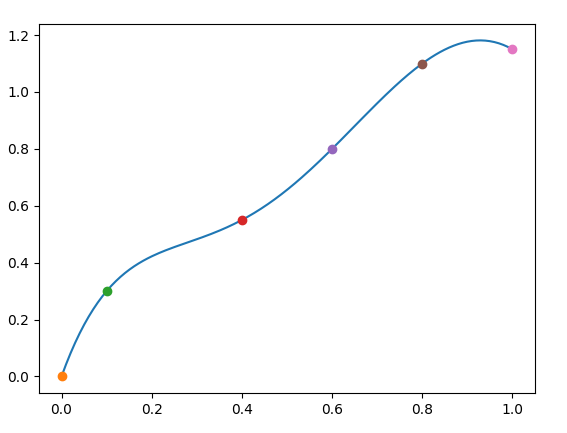
\includegraphics[width=7.5cm,height=6.5cm]{Newton.png}
			Fig. Polinomio de Newton a partir de la tabla $T$
		\end{center}
		
		Calculando se obtiene que en $t_a$ la $C_B =0.5338970444444444$. Ahora remplazamos por el tiempo $t_b = 0.40$ tiempo minimo y $C_{B-exact} = 0.55$.
		\begin{center}
			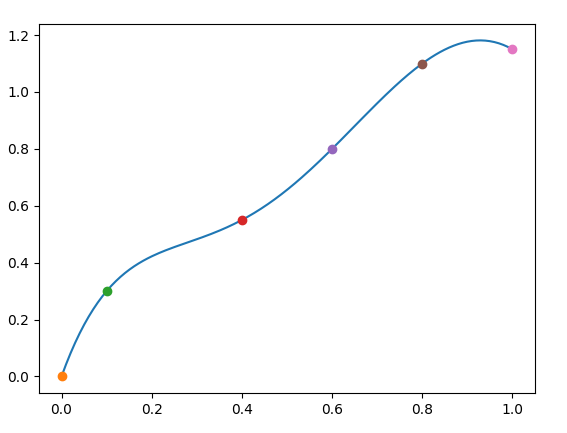
\includegraphics[width=7.5cm,height=6.5cm]{Newton.png}
			Fig. Polinomio de Newton a partir de la tabla $T'$
		\end{center}
		
		Se puede notar que parece ser la misma grafica, pero al calcular la concentracion a partir de $T'$ encontramos que $C_{B-aprox} = 0.5500000000000002$
		
		 
		
		
		
		
		
		
		
		
		
		
		
		El primer metodo en analizar sera Polinomios de Lagrange, utilizando el algoritmo se encontro que para el t=0.82 la $C_B = 1.1217764000000001$ 
		
		\begin{center}
			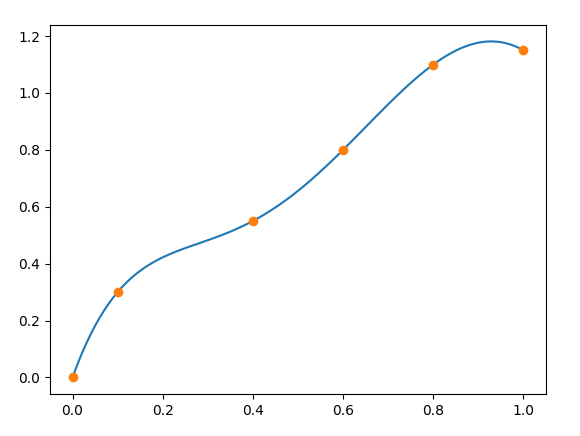
\includegraphics[width=7.5cm,height=6.5cm]{Lagrange.png}
			Fig. Grafica de polinomio usando el metodo de Lagrange
		\end{center}
		
		
		\begin{center}
			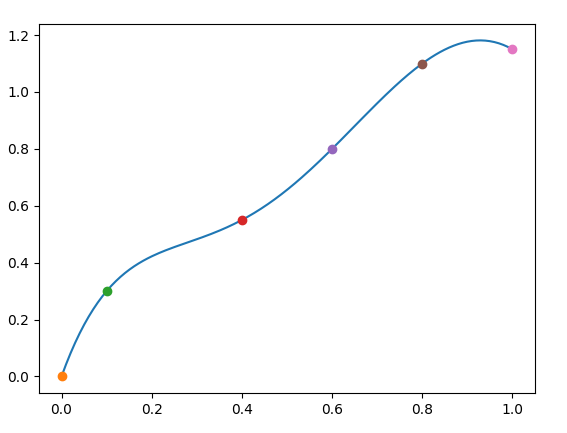
\includegraphics[width=7.5cm,height=6.5cm]{Newton.png}
			Fig. Grafica de polinomio usando el metodo de Newton
		\end{center}
		
		
		\begin{center}
			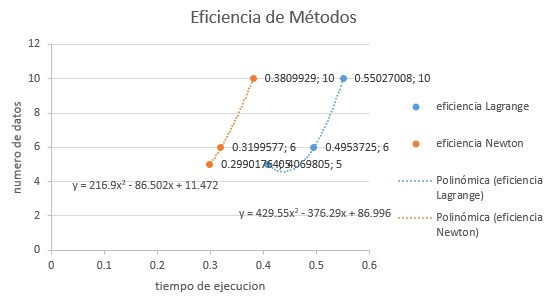
\includegraphics[width=8.5cm,height=6cm]{eficiencia.jpg}
			Fig. Eficiencia entre Lagrange y Newton
		\end{center}
		
		
		\begin{center}
			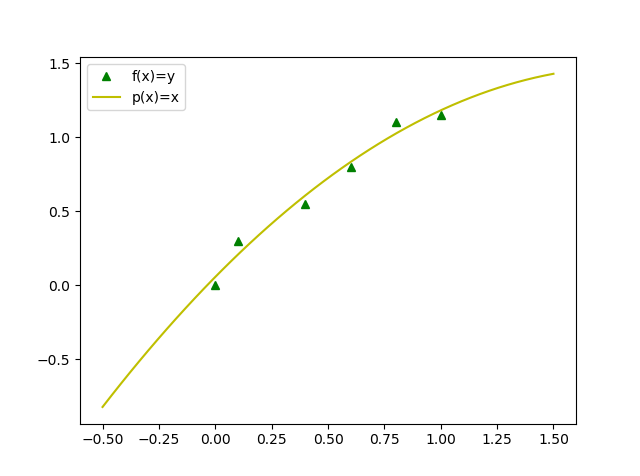
\includegraphics[width=8.5cm,height=7.5cm]{minCuadrados.png}
			
			Fig. Grafica de polinomio usando el metodo de Mínimos Cuadrados
		\end{center}
		
		\noindent {\large \bf 3.2. Analisis de Error}
		
		\vspace*{0.2cm}
		\begin{itemize}
			\item \textbf{Método de Lagrange: } Se
			\item \textbf{Método de Newton: }
			\item \textbf{Aproximación por Minimos Cuadrados:}
		\end{itemize}
		
		\begin{center}
			\renewcommand{\tabcolsep}{10pt}
			\begin{tabular}{ |c|c|c| }
				\hline
				Método            & Tiempo & error  \\ \hline
				Lagrange          & O(n)                & e                      \\ \hline
				Newton            & O(n)                & e                      \\ \hline
				Minimos Cuadrados & O(n)                & e                      \\ \hline \end{tabular}
		\end{center}
		
	
		
		\begin{center}
			{\large \bf 4. OBSERVACIONES}
		\end{center}
		
		- Registrar puntos caracteristicos, aquellos que tengan mayor relevancia en el proceso de experimentación, a partir de estos 
		- Aplicaciones impactantes con interpolacion y minimos cuadrados 
		- Investigaciones realizandose actualmente con interpolacion o minimos cuadrados
		La interpolacion y Minimos cuadrados son la base para muchos investigaciones en ingerieria y ciencias como la fisica, quimica, hasta en temas mas recientes como el Machine Learning, especificamente en las Redes neuronales donde se usa los minimos cuadrados para encontrar el valor de la conexión entre neuronas al momento del entrenamiento.
		
		
		-Si se tiene 2 intervalos $[a' < b'] < [a , b] $ y se realiza la interpolación en cada una, entonces se aproxima mejor en $[a'< b']$ que en $[a < b]$.
		
		- Comparar la data de problema con otra data de mayor tamaño.
		- Puntos caracteristicos: aquellos que describan mejor a la curva, puntos como el maximo, minimo, puntos de inflexion en la función. Estos se optiene de replicar muchas veces el experimento.
		
		Cuando mayor es la cantidad de puntos mayor sera la aproximación.
		
		- Combinacion de ambos metodos, encontrar el polinomio con interpolacion polinomial, luego generamos mas puntos adicionales, luego lo ajustamos con minimos cuadrados, Talvez genera mejores resultados.
		
			
		\noindent Para resolver el problema se implementará una \textbf{interfaz gráfica} donde el usuario pueda elegir el método numérico para resolver el problema, además podrá hallar la $C_B$ en el cualquier tiempo $t$.  
		
		\noindent Con esto es usuario podrá comparar la eficiencia de los diferentes métodos numéricos ver cual es el mejor y el peor, también podrá insertar sus datos para un mayor aprendizaje, ya que la \textbf{eficiencia de los métodos} depende del problema y por ende de los datos.
		
		\begin{center}
			{\large \bf 5. CONCLUSIONES}
		\end{center}
		
		\begin{center}
			{\large \bf Agradecimientos}
		\end{center}
		Los autores agradecen a las autoridades de la Facultad de Ciencias de la Universidad Nacional de 
		Ingenier\'{\i}a por su apoyo.
		%\begin{center}
		%{\large \bf Apendice: }
		%\end{center}
		
	\end{multicols}
	\newpage
	
	\begin{center}
		-----------------------------------------------------------------------------
	\end{center}
	\begin{multicols}{2}
		\begin{list}{}{\setlength{\topsep}{0mm}\setlength{\itemsep}{0mm}%
				\setlength{\parsep}{0mm}\setlength{\leftmargin}{4mm}}
			%
			%------------------------------------- References --------------------
			\small
			\item[1.] Jaan Kiusalaas, \textit{Numerical Methods in Engineering\linebreak with python.} Cambrige University Press \textbf{37} (2010).
			\item[2.] L.Héctor Juaréz V., \textit{Análisis Númerico} Universidad Autónoma Metropolitana \textbf{2008} (2010).
			\item[3.] W. Kincaid, D. Cheney, \textit{Métodos Númericos y Computación,} sexta edición. Cengage Learning, 300-305.
			
			\item[4.] Walter Mora F.,
			\textit{Introducción a los Métodos Numéricos,} primera edición. Instituto Tecnológico de Costa Rica, 2013.
			
			\item[5.] Dr. Herón Morales Marchena,
			\textit{Interpolación, Diferenciación e Integración Numérica,} http://biblioteca.uns.edu.pe/saladocentes/archivoz/cu\\rzoz/cuaderno\_2.pdf.
			
			\item[6.] Pontificia Universidad Católica del Perú, 2011
			\textit{Química General,} http://corinto.pucp.edu.pe/quimicageneral\\/unidades-q2/unidad-2-cinetica-quimica.html.
			%---------------------------------------------------------------------
			%
		\end{list}
	\end{multicols}
\end{document}%\grid